% F088｜末位为 5 的平方及首同尾合十速算｜03_proof.tex
% 继承上传模板的 LaTeX 环境；当前条目的内容独立编写。
\clearpage
\begin{proofbox}
\textbf{\textcolor{CProof}{证明一（最低门槛）：直接展开}}
\par\medskip
\begin{center}
% F088｜algebra 原创简明教学示意图
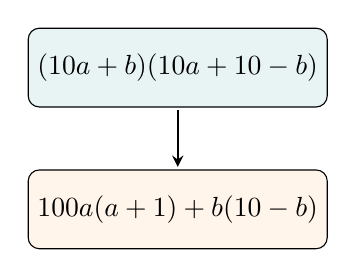
\begin{tikzpicture}[>=stealth,scale=.9]
\node[draw,fill=teal!9,rounded corners,minimum height=1cm] at (4,0){$(10a+b)(10a+10-b)$};
\draw[->,thick] (4,-.6)--(4,-1.4);
\node[draw,fill=orange!8,rounded corners,minimum height=1cm] at (4,-2){$100a(a+1)+b(10-b)$};
\end{tikzpicture}

\end{center}
\medskip
\[(10a+5)^2=100a^2+100a+25=100a(a+1)+25.\]例如 $a=9$，得 $95^2=100\times9\times10+25=9025$。
\end{proofbox}
\clearpage
\begin{proofbox}
\textbf{\textcolor{CProof}{证明二（最快）：平方差}}
\par\medskip
\begin{center}
% F088｜five 原创简明教学示意图
\begin{tikzpicture}[>=stealth,scale=.95]
\node[draw,rounded corners,fill=teal!9,minimum width=2.7cm,minimum height=1cm] (a) at (0,0) {$65^2$};
\node[draw,rounded corners,fill=orange!9,minimum width=3.4cm,minimum height=1cm] (b) at (4.2,0) {$6\times7\mid25$};
\node[draw,rounded corners,fill=teal!15,minimum width=2.7cm,minimum height=1cm] (c) at (8.2,0) {$4225$};
\draw[->,thick] (a)--(b);\draw[->,thick] (b)--(c);
\node at (4.2,-1){\small 前面乘下一个，后面写 $25$};
\end{tikzpicture}

\end{center}
\medskip
\[(10a+5)^2=(10a)(10a+10)+5^2=100a(a+1)+25.\]记住“前一数乘后一数，再接25”，就记住了完整的推导。
\end{proofbox}
\clearpage
\begin{proofbox}
\textbf{\textcolor{CProof}{证明三（最能迁移）：推导首同尾合十}}
\par\medskip
\begin{center}
% F088｜pair 原创简明教学示意图
\begin{tikzpicture}[>=stealth,scale=.95]
\node[draw,fill=teal!8,rounded corners] (a) at (0,0) {$23\times27$};
\node[draw,fill=orange!8,rounded corners] (b) at (4,0) {$2\times3\mid3\times7$};
\node[draw,fill=teal!15,rounded corners] (c) at (8,0) {$621$};
\draw[->] (a)--(b);\draw[->] (b)--(c);
\node at (4,-1){\small 十位相同，个位和为 $10$};
\end{tikzpicture}

\end{center}
\medskip
展开：\[(10a+b)(10a+10-b)\]$=100a^2+100a+b(10-b)$ $=100a(a+1)+b(10-b)$。只需认出两数同十位且个位合十。
\end{proofbox}
